\fancyhead[RE,LO]{\sffamily {\large\textbf{Improving the Reliability of Trapped Ion Quantum Computers}}}

{%\small
	\vspace*{-2.em}
	The weird world of quantum physics may be the next breakthrough in computation. But what can quantum computers do that classical ones cannot? Exploiting their unique properties we can create more efficient algorithms for many computational challenges. The most well known example is integer factorisation for which the runtime on classical computers scales as an exponential function of the size of the number being factorised. This exponential increase however can be overcome by using Shor's algorithm, which can only be implemented on quantum computers.
	
	A classical computer's internal state can be represented as a series of bits, each of which can be $0$ or $1$. The difference in quantum computers is that it stores data in qubits, the quantum analogue of the bit. While only measured as either $0$ or $1$ the outcome of measuring a qubit is probabilistic and in between measurements we can manipulate these probabilities. This state where we are uncertain about the state we'll see when we measure the qubit is referred to as superposition. The most important thing however is that this probability can also be conditional on the state of other qubits in our computer, which is referred to as entanglement. As an example, with two qubits one can create something called a Bell state, where there is an equal probability of measuring each qubit as $0$ or $1$, but either of them is measured $0$ then the other one will be guaranteed $0$ as well. Conversely, if either of them is measured as $1$, then the other will be $1$.
	
	\begin{wrapfigure}{r}{0.4\linewidth}
		\centering
		\vspace*{-0.75em}
		\hspace*{-0.5em}
		\begin{tabular}{c}
			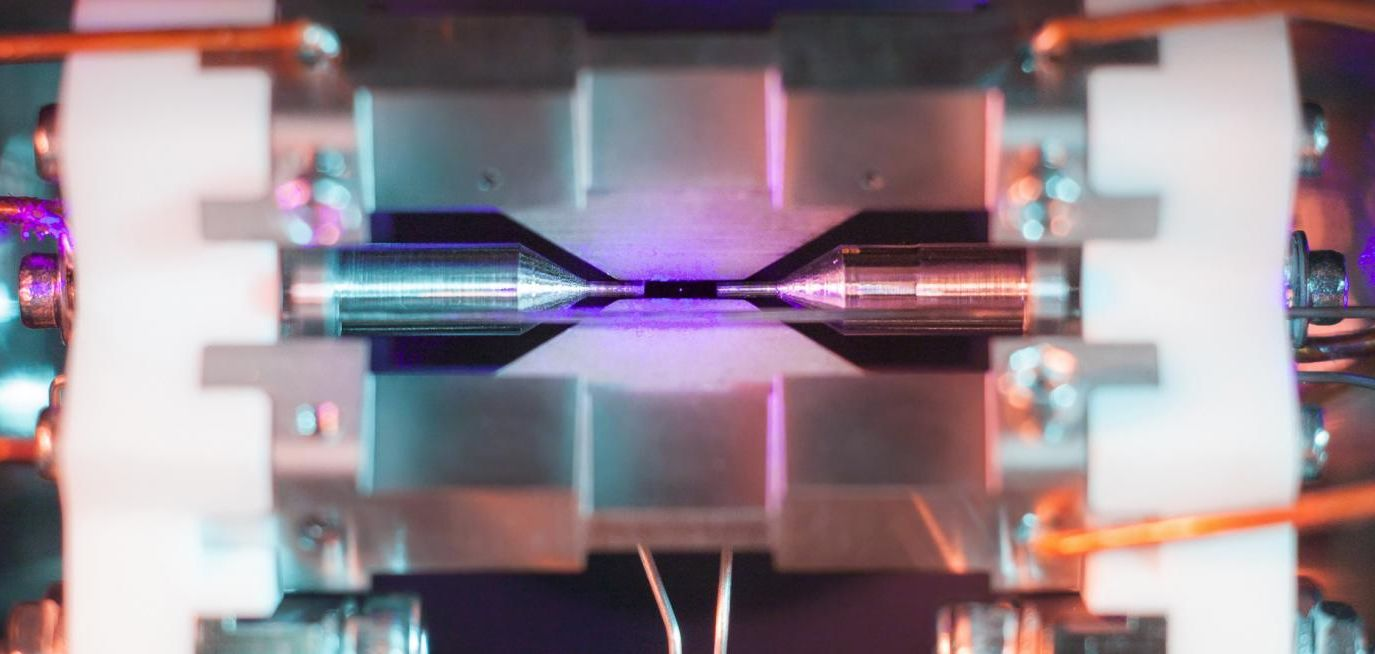
\includegraphics[width=0.95\linewidth]{TIQC.jpg}\\
			\vspace*{-.5em}\\
			\parbox{\linewidth}{\centering\footnotesize A trapped ion at the University of Oxford Ion trap quantum computing research group. Picture taken from their website\footnotemark.}
		\end{tabular}
		\vspace*{-0.75em}
	\end{wrapfigure}
	
	It is very important therefore to ensure that the qubits can be manipulated reliably. To achieve this one needs a relatively stable quantum state that can be used as the qubits and some stable way of sharing information between, manipulating and measuring these qubits to implement quantum algorithms reliably. A promising avenue toward implementation is by using trapped ions. These are charged atomic particles that are confined using magnetic and electric fields. Their internal electronic structure is ideal for use as qubits, while their back and forth motion in the trap is shared between all the ions present. As these ions are cooled to a few millionths of a Kelvin above absolute zero, this motion takes on a quantum nature, meaning that the ions' motion will only have discrete energies. This makes it a very convenient way of facilitating entanglement between them. Combination of Lasers addressing the ions can then be used to facilitate transfer between the various qubit states.
	
	In our MSci project, we simulated how different combinations of lasers, called driving schemes, can improve the reliability of a quantum computer. We did this to set expectations and give guidance to an upcoming experiment, where these schemes will be tested on a physical system. Because of this our main focus was how we can mitigate against experimental errors that inevitably arise and reduce the reliability of the qubits' state. These come from a variety of sources like the temperature and degree to which the ions can be confined. To find the best setup for the experiment we evaluated different driving schemes aimed to address the specific problems a physical system might face and have given recommendation on which ones to use. We also shown that several of these schemes could be combined giving improved performance. We hope that the increased reliability of these schemes will be demonstrated in the following years.
}
\vspace*{\fill}

\footnotetext[1]{\href{https://www.physics.ox.ac.uk/research/group/ion-trap-quantum-computing}{https://www.physics.ox.ac.uk/research/group/ion-trap-quantum-computing}}
\newpage

\fancyhead[RE,LO]{}